%%%%%%%%%%%%%%%%%%%%%%%%%%%%%%%%%%%%%%%%%%%%%%%%%%%%%%%%%%%%%%%%%%%%
%% I, the copyright holder of this work, release this work into the
%% public domain. This applies worldwide. In some countries this may
%% not be legally possible; if so: I grant anyone the right to use
%% this work for any purpose, without any conditions, unless such
%% conditions are required by law.
%%%%%%%%%%%%%%%%%%%%%%%%%%%%%%%%%%%%%%%%%%%%%%%%%%%%%%%%%%%%%%%%%%%%

\documentclass{beamer}
\usetheme[faculty=science, university=uu, logo=uu-logo]{fibeamer}
\usepackage[utf8]{inputenc}
\usepackage[
  main=francais
]{babel}
\title{Le Cas PAPCAR} %% that will be typeset on the
\subtitle{Diagnostic et Réingénierie des Processus avant la mise en œuvre d’un ERP} %% title page.
\author{Vincent Cadenet, Hugo Fougeres, Ludovic Fritel, Alexander Hoffmann, Jeremy Roca}
\usepackage{ragged2e}  % `\justifying` text
\usepackage{booktabs}  % Tables
\usepackage{tabularx}
\usepackage{tikz}      % Diagrams
\usetikzlibrary{calc, shapes, backgrounds}
\usepackage{amsmath, amssymb}
\usepackage{url}       % `\url`s
\usepackage{listings}  % Code listings
\frenchspacing
\begin{document}
  \frame{\maketitle}

  \AtBeginSection[]{% Print an outline at the beginning of sections
    \begin{frame}<beamer>
      \frametitle{Table des matières partie \thesection}
      \tableofcontents[currentsection]
    \end{frame}}

    \section{La lettre du client mécontent}
    \subsection{Les griefs relevés par le client}
    \begin{frame}{Les griefs relevés par le client}
      \begin{itemize}
      	\item Temps d’attente important
		\item Rupture de stock
		\item Absence de date de livraison
		\item Réception d’une ancienne facture
		\item Communication avec le client sous-optimal
		\item Réception d’un nouveau un bon de commande
		\item Impossibilité de parler au responsable (absent)
		\item Peu de clarté dans les informations fournies
      \end{itemize}
    \end{frame}

	\subsection{Dysfonctionnements dans l'entreprise}
    \begin{frame}[label=lists]{Dysfonctionnements dans l'entreprise}
      \framesubtitle{}
      \begin{itemize}
      	\item Manque de communication entre les services
      	\item Organisation sous-optimale en cas d'absence des responsables
      	\item Certaines commandes ne semblent pas être prises en compte
      	\item Problèmes sur la gestion des stocks
      \end{itemize}
    \end{frame}
    
    \subsection{Axes d'amélioration}
    \begin{frame}[label=lists]{Axes d'amélioration}
      \framesubtitle{}
      \begin{itemize}
      	\item Améliorer les compétences de communication avec les clients
      	\item Organiser les absences des responsables
      	\item Etablir un système permettant de voir les stocks en temps réel
      \end{itemize}
    \end{frame}

	\section{Etude de la vente sur stock}
	\subsection{Processus de la vente sur stock}
    \begin{frame}[label=lists]{Processus de la vente sur stock}
      \framesubtitle{}
      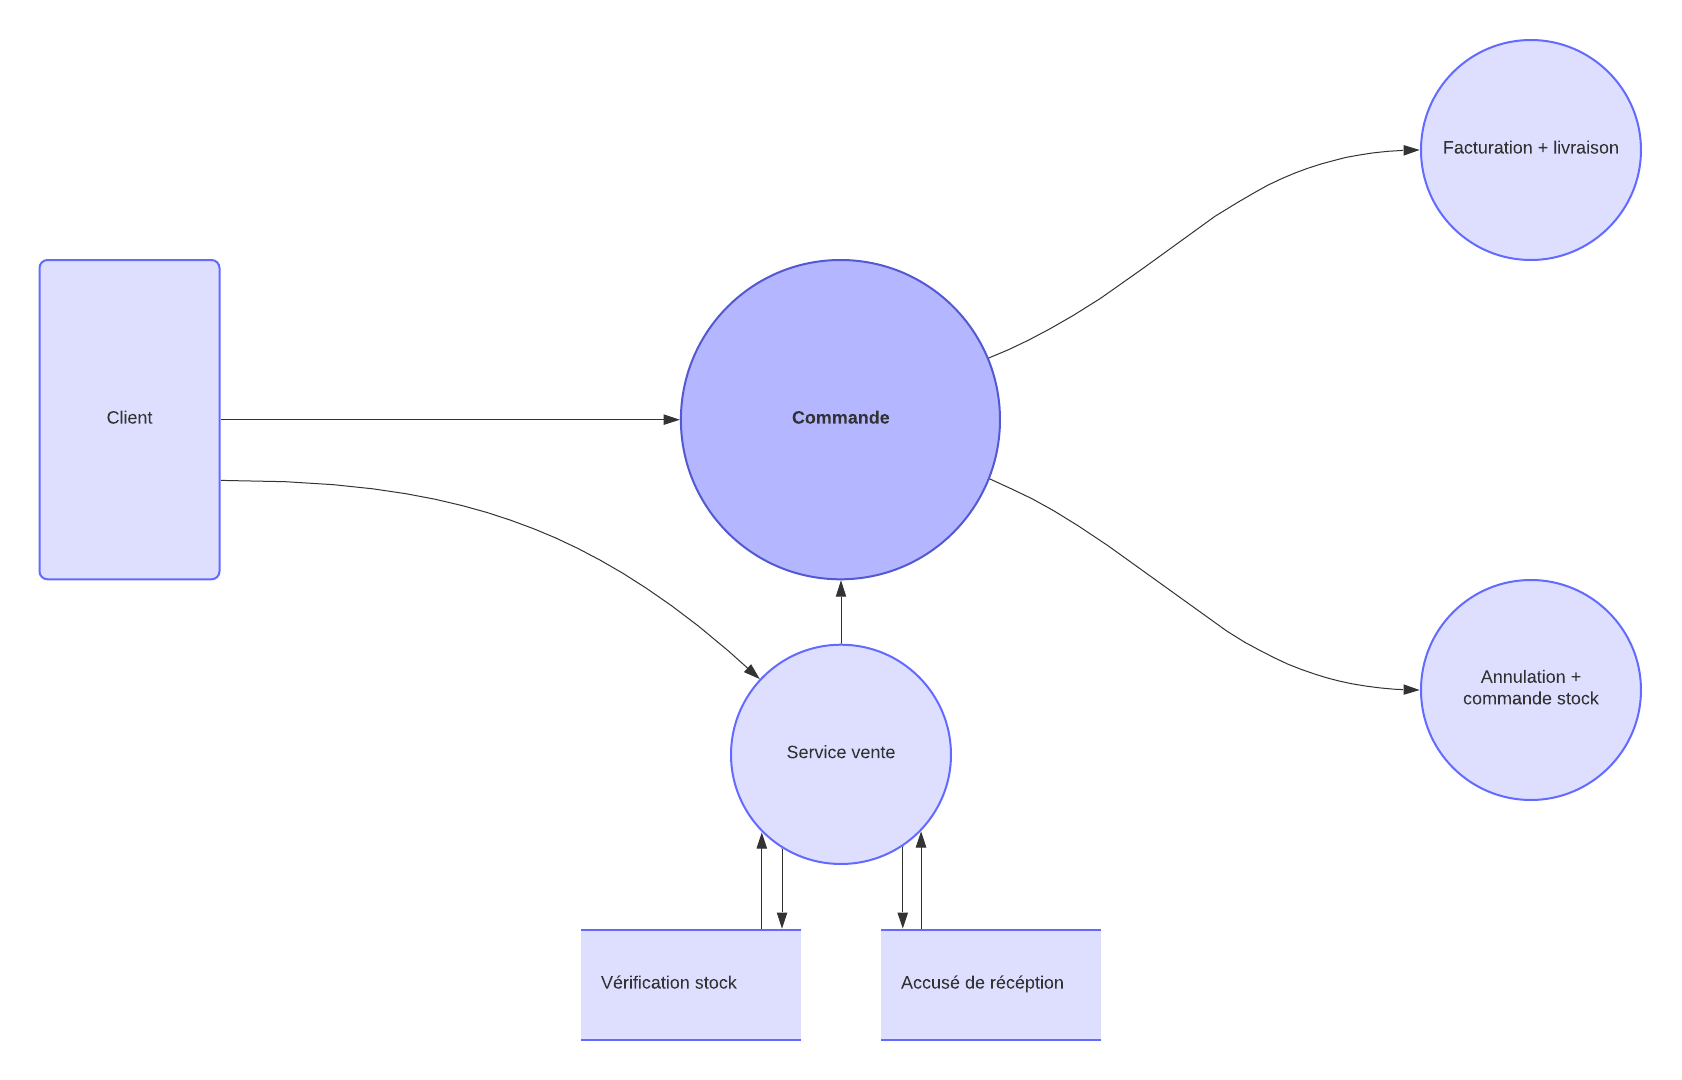
\includegraphics[width=100mm]{resources/flow}
    \end{frame}
    
    \subsection{Optimisation du processus}
    \begin{frame}[label=lists]{Optimisation du processus}
      \framesubtitle{}
      \begin{itemize}
		\item Capacité de prise de commande sur internet
		\item Accusé de réception
		\item Accès et communication avec un responsable
		\item Traçabilité des commandes effectuées par chaque client
		\item Amélioration du service de ticketing support
		\item Rajout de l’effectif au service support
		\item Mise à jours des stocks en temps réel
		\item Facturation lors de l’expédition
      \end{itemize}
    \end{frame}

\end{document}
